
\chapter{$O^2$ Simulations of T0+ A-side}
The ALICE Online-Offline Computing System $O^2$ has built-in simulation capabilities which include the generation of events and the transport of particles from the primary vertex. Using the FIT detector geometry in a simulation, we can determine the number of particles that can be detected using FIT sensitive components, and the number of secondary particles that contribute to the noise of other detectors. $O^2$ handles simulation data very similarly to true event data in the form of \textit{digits}, which only keep the location and energy deposition in the detector channel. Using this information, simulations can be used to inform live track reconstruction, background estimation, and particle identification. 


\section{Monte Carlo Event Simulations and Detector Geometry}

\subsection{Geant}
Run 3 requires fast Monte-Carlo simulations to meet the requirements of analysis topics. Particle transport must be optimized to handle an increase by a factor of 20 in simulation requirements. To do this, Geant4 has a multi-threading transport package that satisfies these requirements \cite{Geant4}. Along with the particle transport efficiency, Geant4 has compatibility with ROOT geometry capabilities that allow for construction of ALICE detector geometry in simulation. This helps to accurately track which of the detectors are hit, which materials a particle travels through, and it informs the MC generator of the probability distributions for interactions between beam particles and ALICE components. HIJING produces jets at the interaction point that are propagated through the detector. 

\begin{figure}[H]
    \centering
    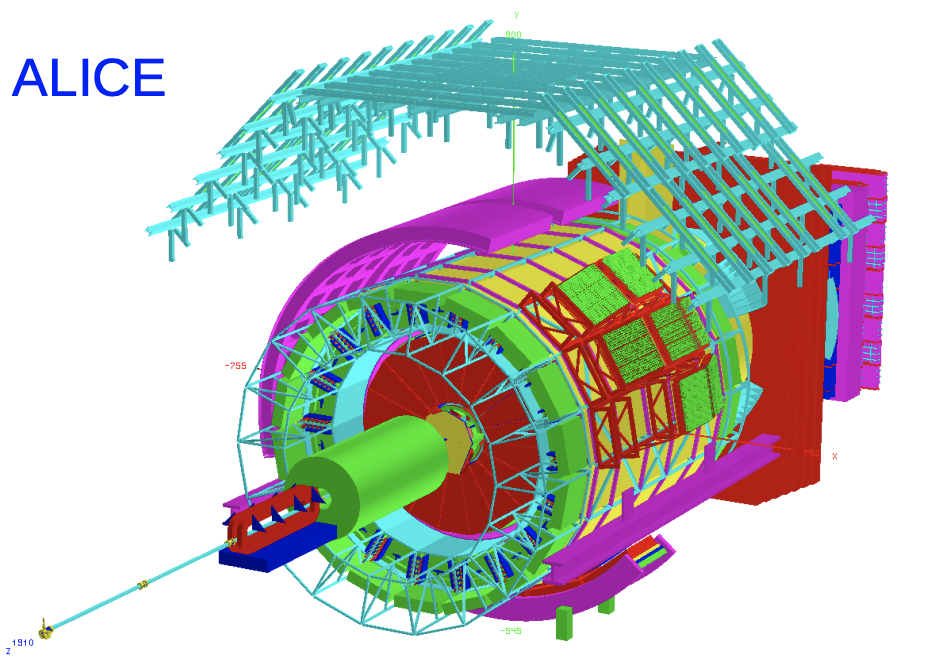
\includegraphics[width=0.6\textwidth]{figures/ALICE/GEANT_Geometry.png}
    \caption{ALICE detector geometry implemented in Geant4}
    \label{fig:GEANT_Geometry}
\end{figure}


\sectionWithFixedHeader{T0+ Aluminum Support Structure $O^2$ Implementation}{T0+ Support Structure}
CAD drawings of the final design for FIT T0+ A-side support structure were completed in summer of 2019, and the support structure needed to be included in the simulation geometry. Using Root geometry, the structure was implemented into the $O^2$ FT0 class, and is now included in simulations of FIT T0+. 

\begin{figure}[H]
    \centering
    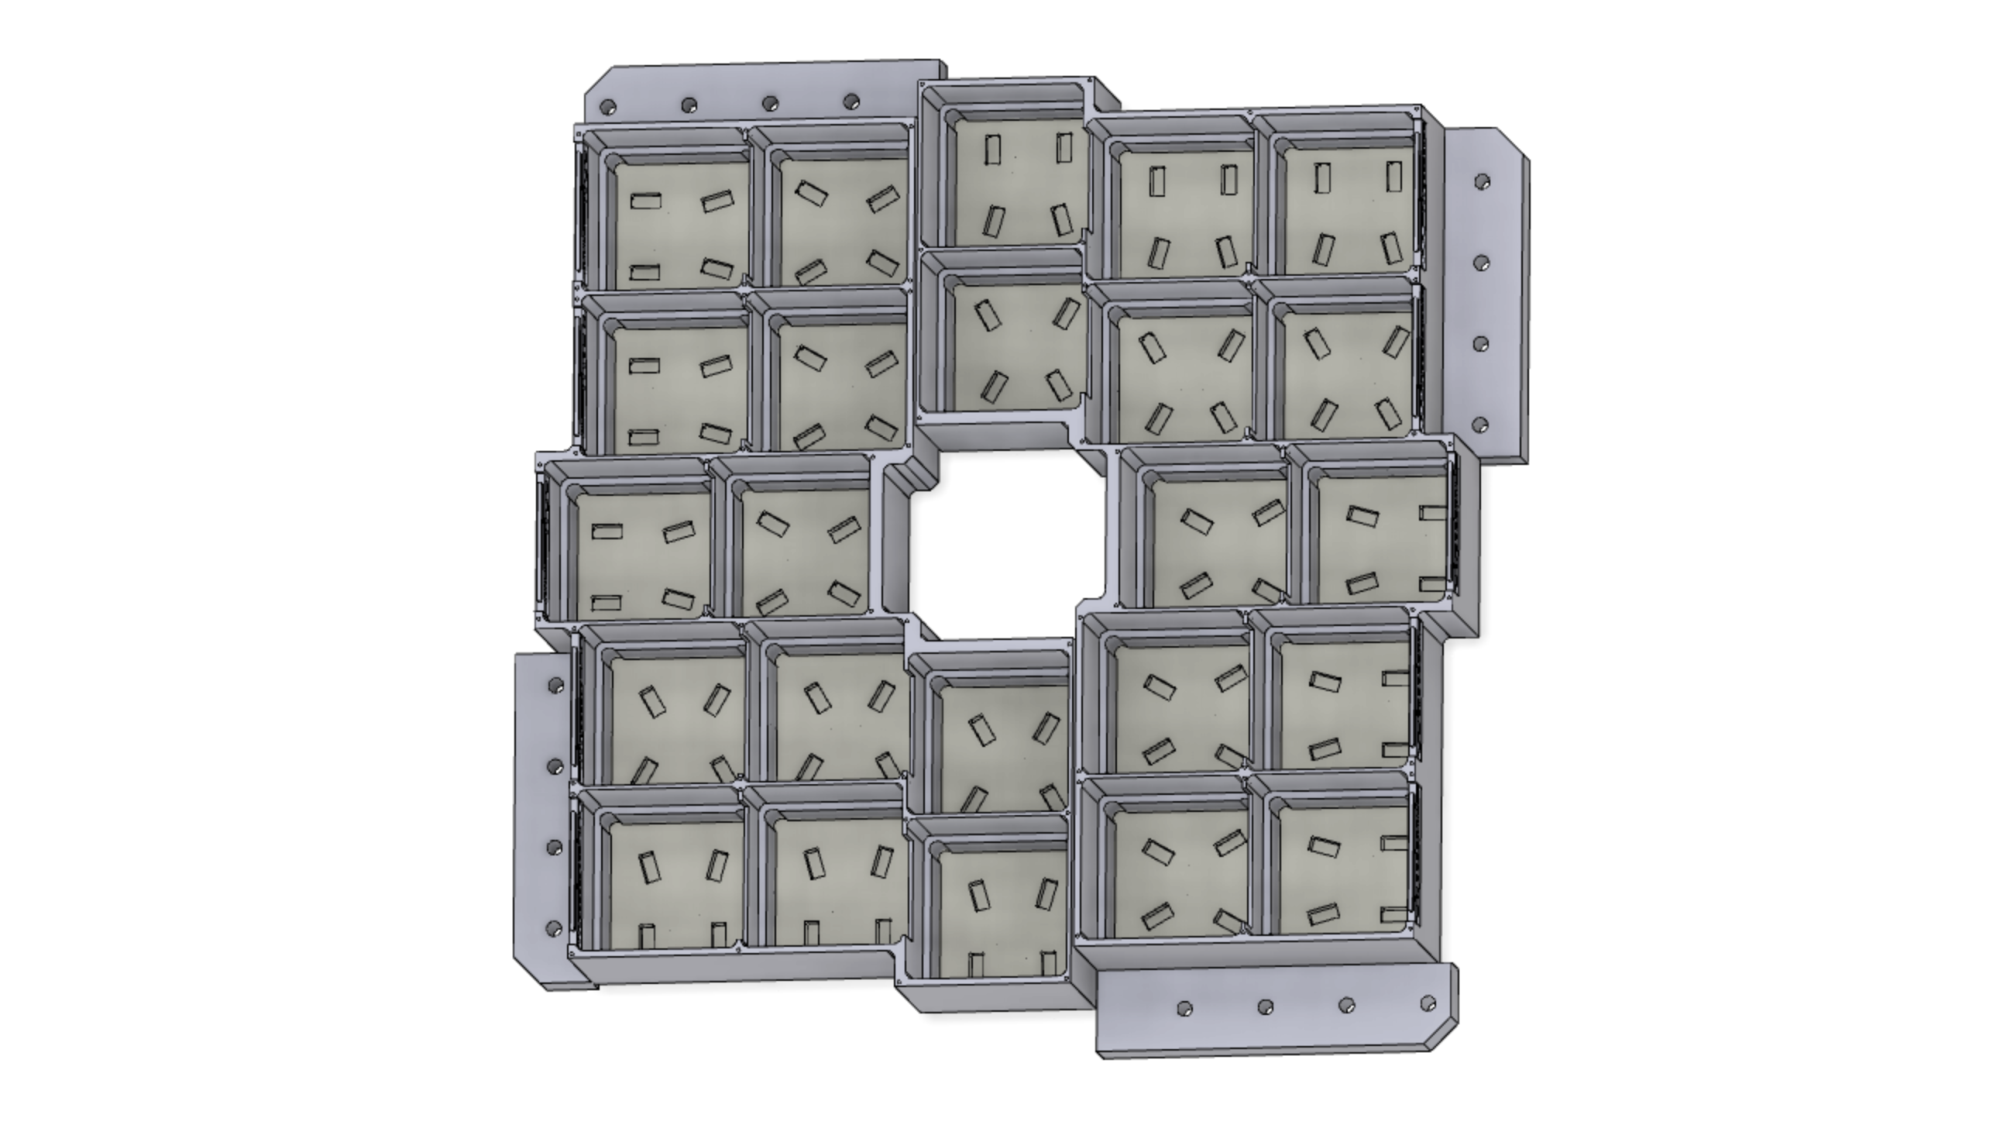
\includegraphics[width=0.6\textwidth]{figures/FIT/FIT_Support_Structure_CAD.pdf}
    \caption{CAD drawing of Aluminum support structure for T0+ A-side.}
    \label{fig:FT0_CAD}
\end{figure}

\begin{figure}[H]
    \centering
    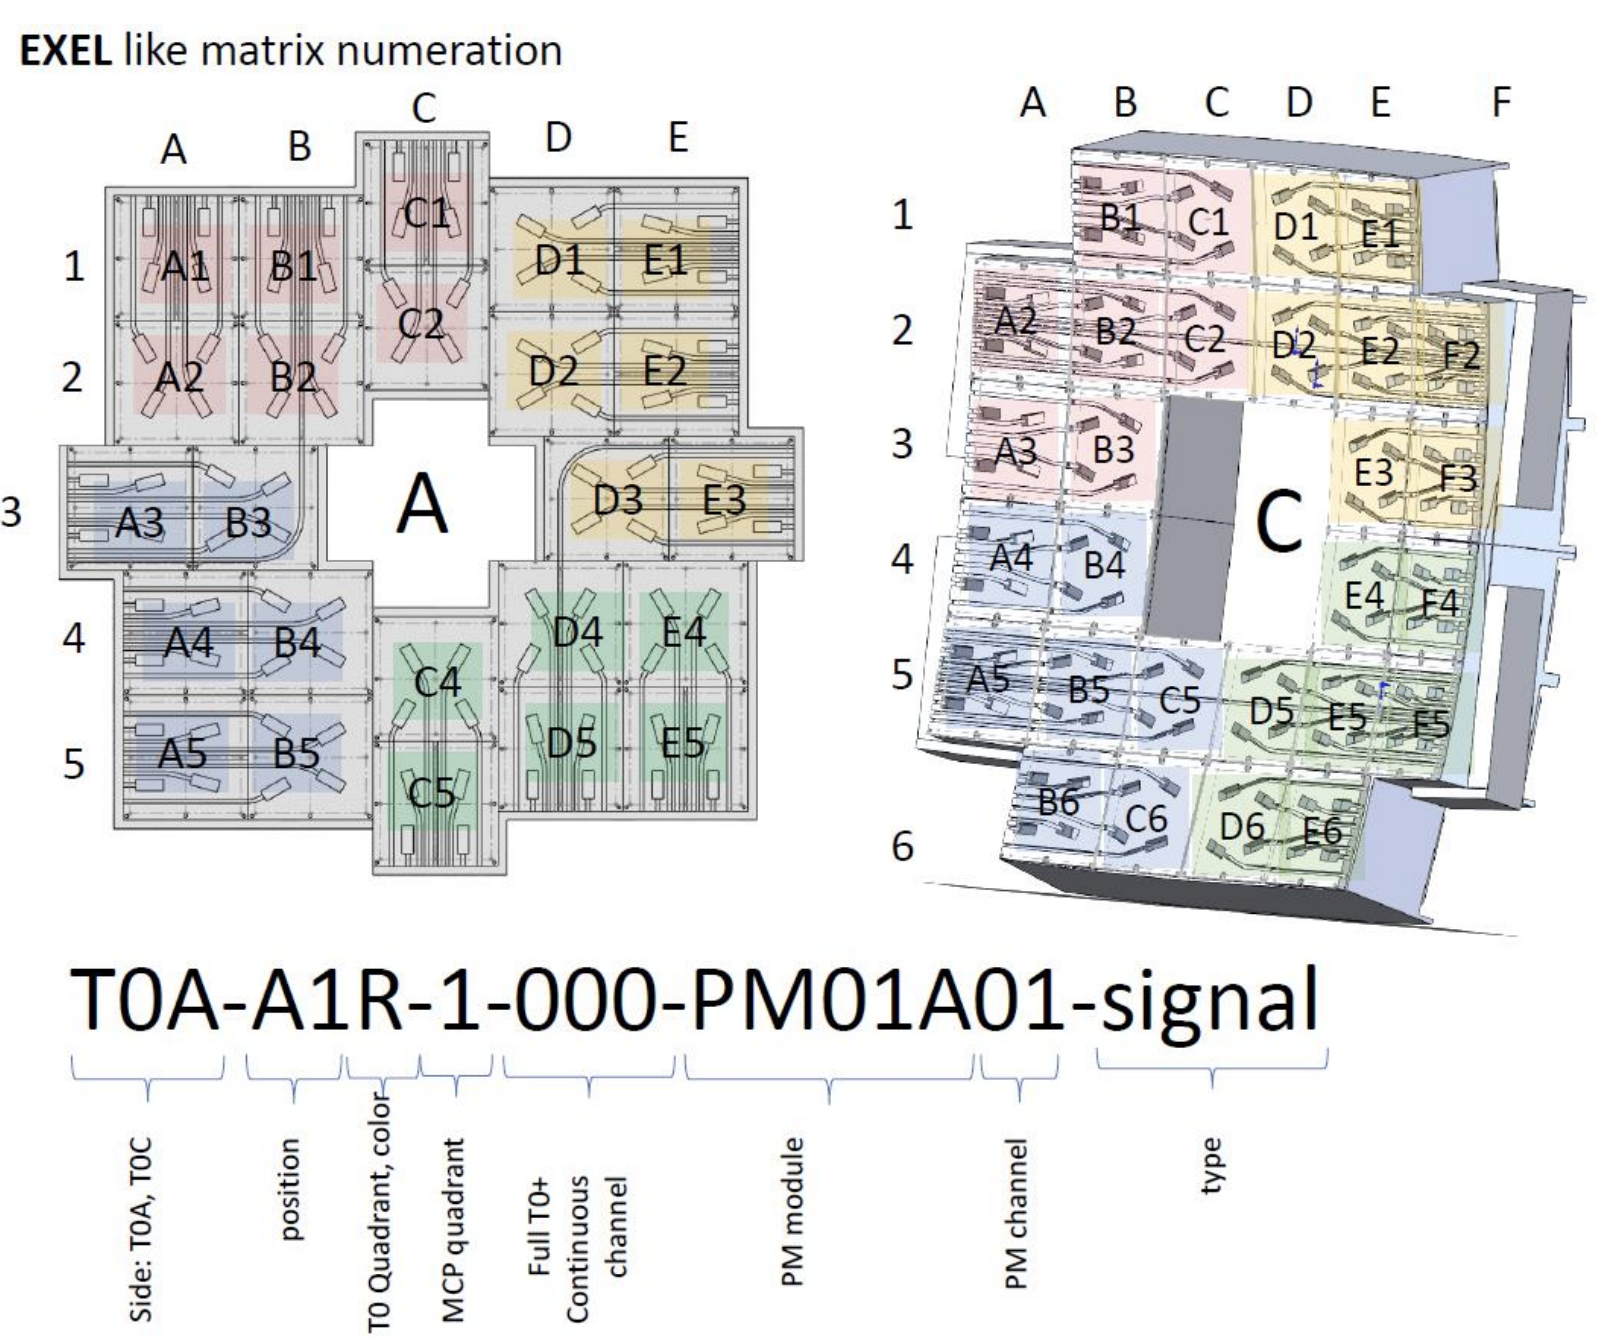
\includegraphics[width=0.8\textwidth]{figures/FIT/T0_Structure_and_Cell_Numbers.png}
    \caption{Aluminum support structure for T0+. Cells are enumerated by row and column.}
    \label{fig:FT0_Labels}
\end{figure}

\section{Simulations}
\subsection{Example Analysis: T0+ A-side Sensitive Components}
\begin{figure}[H]
    \centering
    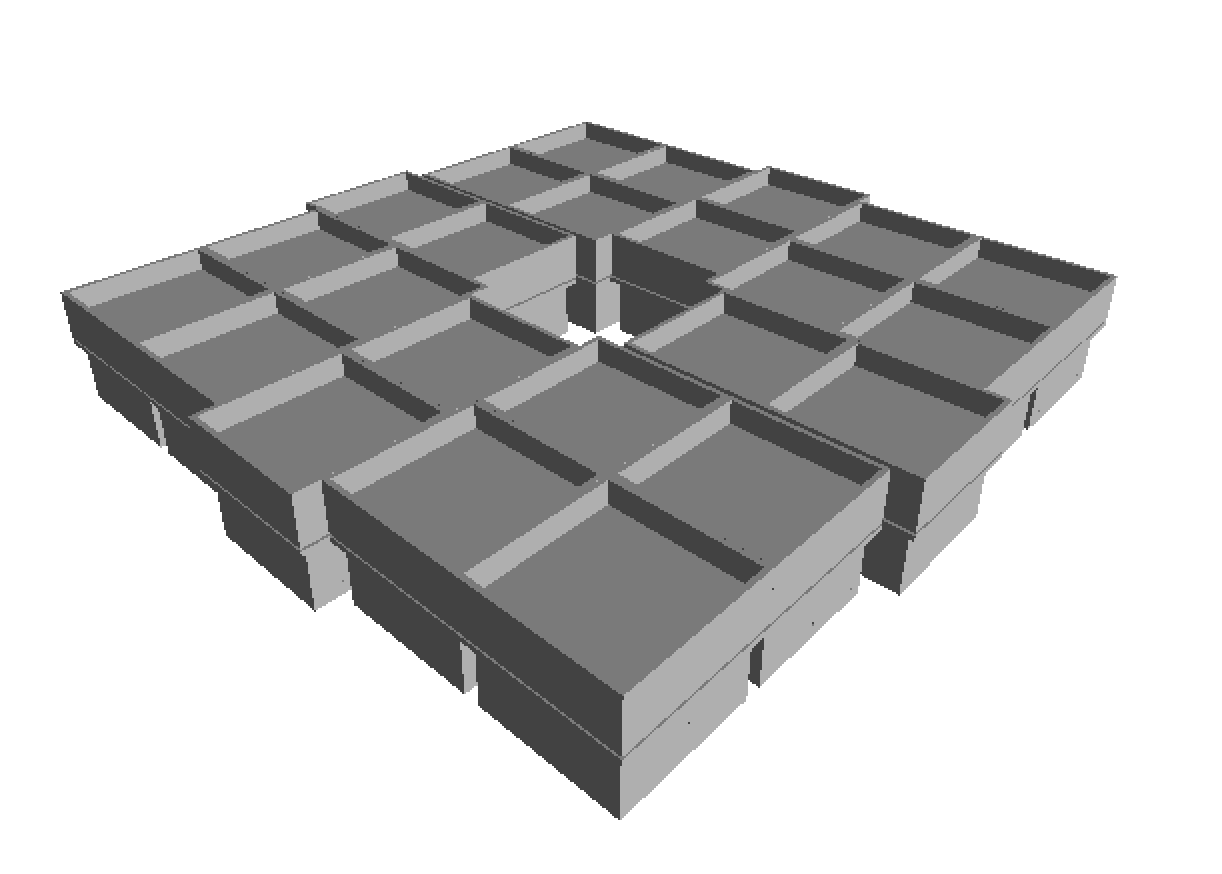
\includegraphics[width=0.8\textwidth]{figures/FIT/T0+_Sensitive_Components.png}
    \caption{Sensitive components for T0+ A-side. This includes the Cherenkov radiative crystals (Top) and PMTs (Bottom), coupled with optical grease}
    \label{fig:my_label}
\end{figure}

\begin{figure}[H]
    \centering
    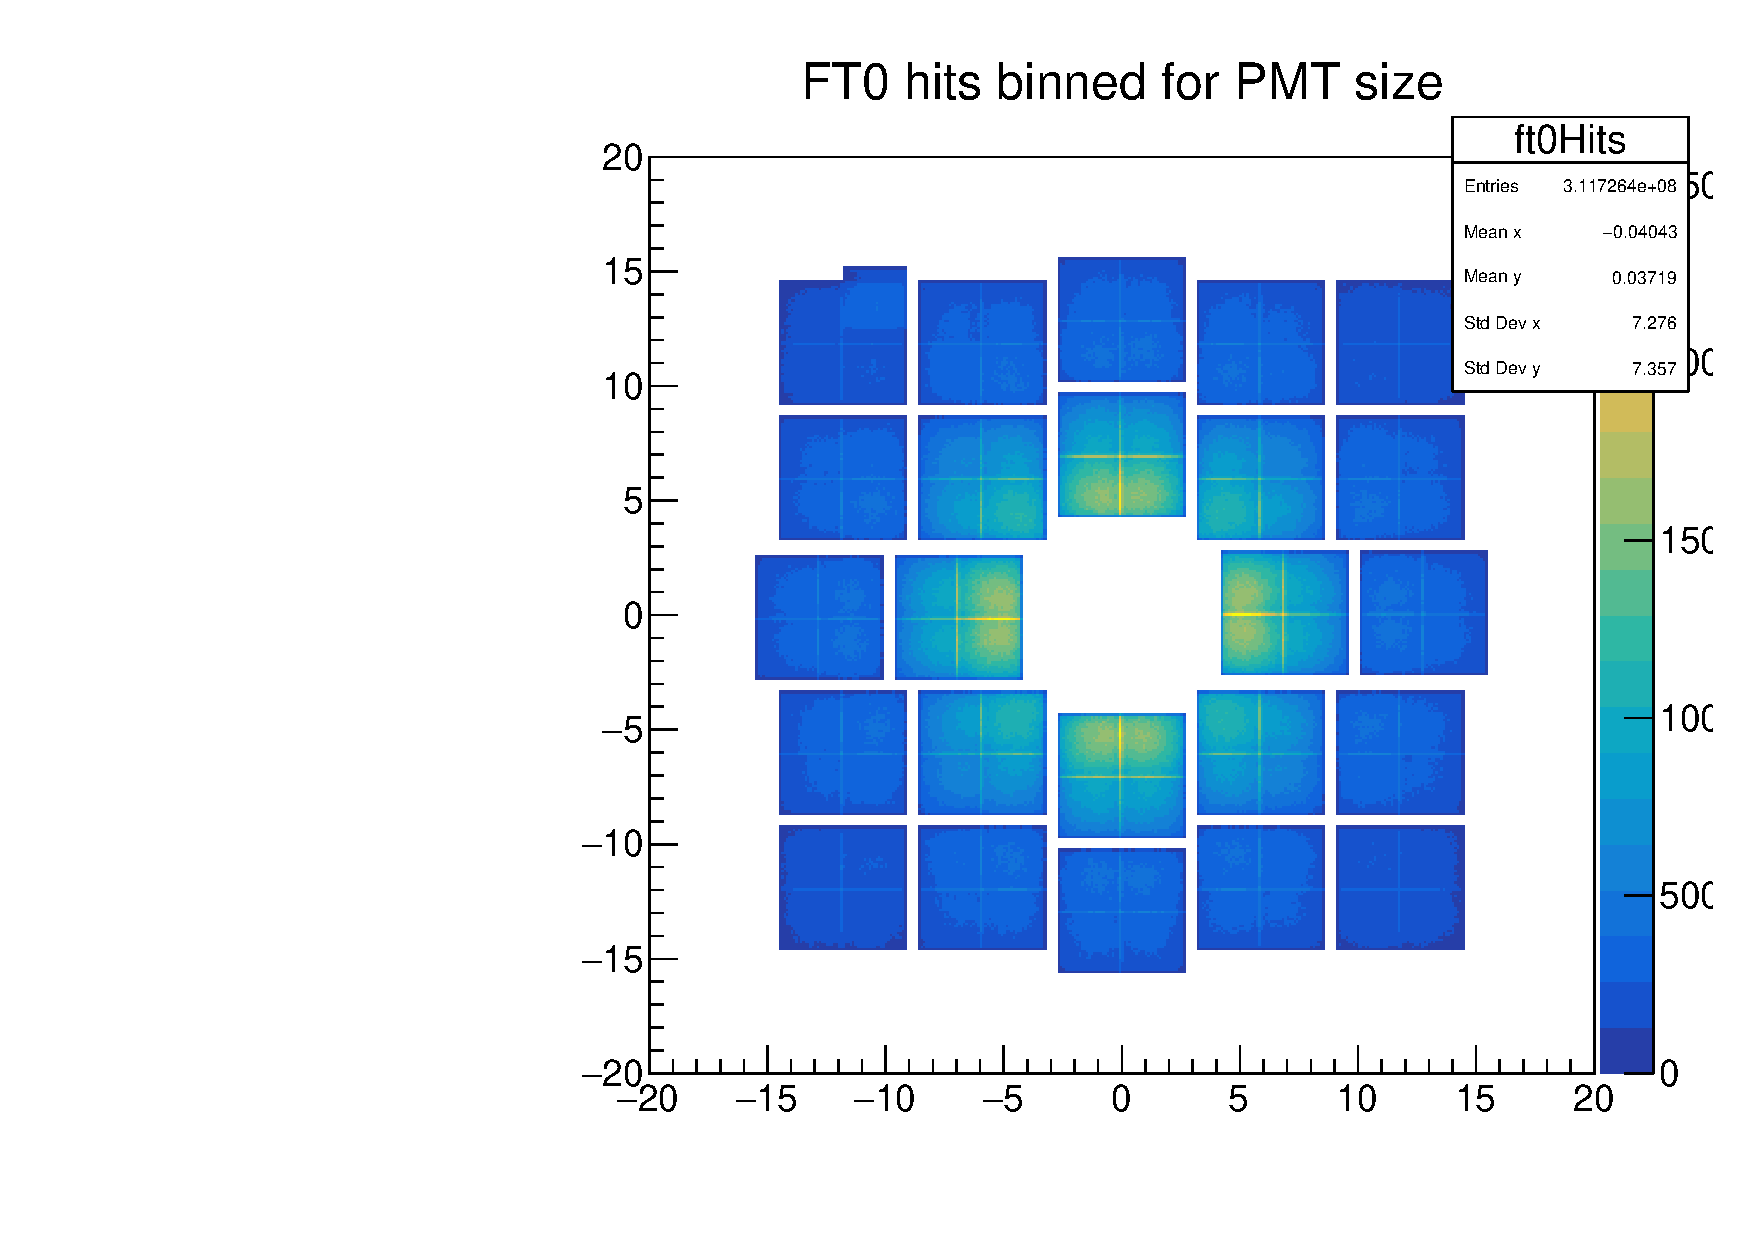
\includegraphics[width= 0.8\textwidth]{figures/analysis/T0+_Sensitive_Components.pdf}
    \caption{Histogram binned for PMTs on the FIT T0+ A-side sensitive components}
    \label{fig:sensitive_components}
\end{figure}
